\documentclass{article}
\usepackage{enumitem,amsmath,amssymb,tikz,graphicx}

\title{MAT 211: Homework \#1}
\date{January 2026}
\author{-Your Name Here-}
\begin{document}
\maketitle 

Use Overleaf or a similar LaTeX editor to write up your answers to the following questions.  Save all pages to a single multi-page PDF and upload to Canvas.

\section*{Types of Reasoning and Set Theory}

\begin{enumerate}

\item Define the terms \emph{inductive reasoning} and \emph{deductive reasoning} as explained in class and in the course videos.

\item Consider the following terms as used in class and course videos:
\begin{enumerate}
    \item Explain how \emph{math} and \emph{science} are distinguished, based on class discussion and course videos.
    \item Define the terms \emph{theorem} and \emph{theory}, as discussed in class and in the course videos.
\end{enumerate}

\item Consider the set \(S= \{\mathbb{R},\{\mathbb{Q},\mathbb{N}\}\}\).  List all subsets of \(S\).

\item Let \(A\) =  \(\{b,c,d\}\).  How many elements are in the power set of \(A\)? Let \(\mathcal{P}(A)\) represent the power set of \(A\).  List the elements of \(\mathcal{P}(A)\).


\item Let \(B = \{a,b\}\).  How many elements are in \(\mathcal{P}(B)\)?  List the elements of \(\mathcal{P}(B)\).

\item Let \(A\) = \(\{b,c,d\}\) and \(B\) = \(\{a,b\}\). List the elements of the Cartesian product \(\mathcal{P}[A] \times \mathcal{P}[B].\)

\item 
    \begin{enumerate}
        \item True or False: \( \{1,1,1 \}\in\mathcal{P}(\mathbb{N})\). Explain.  Note that \(\{1,1,1\}\), in this instance, refers to the \emph{list} of consecutive duplicates of the number 1.  
        \item Describe the Cantor Set. Is the Cantor Set an element of \(\mathcal{P}(\mathbb{R}^2)\) ? Note: \(\mathbb{R}^2\) is the Cartesian product of \(\mathbb{R}\) with itself.
    \end{enumerate}

\item Draw and shade a Venn diagram for the set \(A \cap B - C\).

\newpage

\item Write a set theoretic expression (involving operations such as \(\cap\), \(\cup\) or \(-\)) for the following diagram. 

\begin{center}
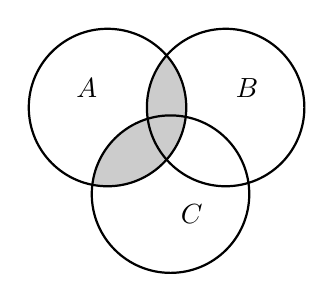
\begin{tikzpicture}
   
 % Shade (A ∩ B) U (A ∩ C)
    \begin{scope}
       \clip (0,0) circle(1); % restrict to A
       \fill[gray!40] (1.5,0) circle(1); % shade A intersect B
       \fill[gray!40] (0.8,-1.1) circle(1); %  shade A intersect C
    \end{scope}

 % Draw the circles
    \draw[thick] (0,0) circle(1) node[above left] {\(A\)}; % Circle A with label
    \draw[thick] (1.5,0) circle(1) node[above right] {\(B\)}; % Circle B with label
    \draw[thick] (0.8,-1.1) circle(1) node[below right] {\(C\)}; % Circle C with label

    
\end{tikzpicture}
\end{center}
\end{enumerate}

\section*{Type Theory and the Curry-Howard Correspondence}
\begin{enumerate}[resume]
  
\item {Russell's Paradox and the Limits of Naive Set Theory}
\begin{enumerate}
    \item Consider the proposed set \(R = \{x : x \notin x\}\), the ``set of all sets that do not contain themselves.'' Explain, in your own words, why asking whether \(R \in R\) leads to a contradiction.
    \item Why does this paradox suggest that we cannot freely form sets using any property we like?
\end{enumerate}

\item {Type Theory as a Foundation in Mathematics}

Russell's Paradox showed that naive set theory needs restrictions. One alternative foundation is \emph{type theory}, where every object belongs to a specific \emph{type}, and types are organized in a hierarchy that prevents problematic self-reference.
\begin{enumerate}
    \item In your own words, explain how requiring objects to have designated types might prevent paradoxes like Russell's.
    \item In Lean, when we write \texttt{n : Nat}, we are declaring that \texttt{n} has type \texttt{Nat} (natural number). Why might a proof assistant benefit from tracking types explicitly?
\end{enumerate}

\item{The Curry-Howard Correspondence (Preview)}
The Curry-Howard correspondence is a foundational idea connecting logic and computer science. 
\begin{enumerate}
    \item In a sentence or two, explain how the Curry-Howard correspondence describes a fundamental connection between these two fields.
    \item In a sentence or two, explain how Lean is both a programming language and a math proof assistant. 
\end{enumerate}
\end{enumerate}

    
\end{document}
